\section{Evaluation}
\label{sec:evaluation}
The experiments evaluate whether scene-conditioned sampling reduces the number of candidate trajectories required for reliable closed-loop planning, and what this costs in trajectory quality and runtime.
The proposed Sparse Planner (SP) is compared with FOP, FISS+, CEM, and MPPI.
FOP provides the uniform-sampling baseline, FISS+ a baseline that accelerates the search over the same grid, and CEM and MPPI adapt their sampling distributions online using cost feedback.
SP without fallback, denoted as SP$^{*}$, is additionally evaluated to isolate the contribution of the learned sampler from that of the fallback mechanism.

\subsection{Experimental Setup}
\label{subsec:setup}
\textbf{Scenarios.}
All methods are evaluated in closed-loop simulation on 26 CommonRoad scenarios covering urban, interurban and highway traffic.
% TODO(author): 6 of these 26 scenarios are part of the CVAE training set and 15 share a map with it; the 11 scenarios
% with an unseen map are evaluated separately in Section V-C. Keep this sentence or replace the test set by a held-out split.
Of these, 11 scenarios use road maps that do not occur in the CVAE training data; they are analyzed separately in \autoref{subsec:ablation}.
A scenario counts as failed if, in any planning cycle, the planner returns no feasible trajectory, or if the ego vehicle comes to a standstill before reaching the goal region, since the simulation does not model standstill.

\textbf{Planner configurations.}
All planners share the trajectory generation, feasibility checks, collision checks, and cost evaluation of FOP, so that they differ only in the sampled terminal parameters $(d, \dot{s}, T)$.
$N$ denotes the number of candidate trajectories per planning cycle.
FOP and FISS+ use grids $N_d \times N_{\dot{s}} \times N_T$ with an odd $N_d$, so that the lane center $d=0$ is always a candidate; the grids $3{\times}2{\times}2$, $3{\times}3{\times}2$, $5{\times}4{\times}3$, $5{\times}5{\times}5$, $7{\times}6{\times}6$, $9{\times}8{\times}7$, and $11{\times}10{\times}9$ (12 to 990 candidates) are reported in the columns $N=8$ to $1024$.
FISS+ evaluates only part of its grid but adds refinement samples, so its evaluated count differs from $N$ (29 to 319 trajectories per cycle on average).
For CEM and MPPI, $N$ is the total budget per cycle, split into $I=\min(8,\max(1,N/8))$ iterations of $N/I$ samples; both start from the previous cycle's solution with an initial standard deviation of 0.3 in normalized parameter coordinates (CEM: elite fraction 0.1, smoothing 0.7; MPPI: temperature 0.1, step size 0.7).
SP draws $N$ samples from the CVAE; if none of them is feasible, the FOP grid $5{\times}5{\times}5$ (125 candidates) is evaluated as a fallback.

\textbf{Metrics.}
For each $N$, the following metrics are reported: the number of failed scenarios $N_{fail}$ (out of 26); the average executed-trajectory cost $\bar{J}$; the average runtime per planning cycle $\bar{t}$; and, for SP, the fallback rate $P_{fb}$, the share of planning cycles in which the fallback is invoked.
Because a failed scenario terminates early, its executed-trajectory cost is not comparable with that of a completed scenario.
$\bar{J}$ is therefore averaged over the scenarios that all methods complete at the respective $N$; the number of these scenarios is given in \autoref{tab:planner_comparison}, and $\bar{J}$ is comparable only within a column.

The cost of an executed trajectory with $K$ time steps of $\Delta t = 0.1$\,s is computed with the cost terms of FISS+~\textcite[cf.][Equation (7)]{Sun2023FISSPLUS}:
\begin{equation}
\label{eq:cost_function}
\begin{aligned}
J_{\mathrm{total}} &= \frac{1}{K}\sum_{k=1}^{K} \Big[
w_V (v_{\mathrm{target}}-v_k)^2
+ w_A \lVert \mathbf{a}_k \rVert^2
+ w_J \lVert \dot{\mathbf{a}}_k \rVert^2 \\
&\quad
+ w_D \max_{i=1,\ldots,o} \xi_{i,k}
+ w_{LC}\, d_k^2 \Big]
+ w_T\, t_f ,
\end{aligned}
\end{equation}
where $v_{\mathrm{target}}=14$\,m/s is the desired velocity, $\mathbf{a}_k$ and $\dot{\mathbf{a}}_k$ are the longitudinal and lateral acceleration and jerk in the Fren\'et frame, $d_k$ is the lateral deviation from the reference path, and $t_f=K\Delta t$ is the duration of the executed trajectory.
The term $\xi_{i,k}=e^{-w_{dist} d_{i,k}}$ penalizes proximity to obstacles, where $d_{i,k}$ is the distance between the ego vehicle and the center of the $i$-th of the $o$ surrounding obstacles.
The weights are $w_V=0.1$, $w_A=10$, $w_J=10$, $w_D=100$, $w_{dist}=0.1$, $w_T=1$, and $w_{LC}=10$.
The obstacle term is used only to evaluate the executed trajectory; the per-cycle planning cost of all planners omits it ($w_D=0$), and obstacles enter planning through the collision check.

\textbf{Implementation and hardware.}
All experiments run on an Intel Core Ultra 9 285K CPU and an NVIDIA GeForce RTX 5070 Ti GPU.
All planners, including the trajectory evaluation and the fallback of SP, are implemented in C++17 (GCC 15.2, \texttt{-O3}) and are invoked from a Python-based CommonRoad simulation via pybind11.
CVAE inference is performed on the GPU using an FP16 TensorRT engine, while all other computations run on a single CPU core, the same configuration as for all baselines.
The reported runtime is the time of the planning call per cycle; it excludes the simulation and the rasterization and preprocessing of the BEV images, which are assumed to be provided by an upstream perception and prediction module.
For SP and SP$^{*}$, it includes CVAE inference, trajectory generation and evaluation, and the FOP fallback whenever it is triggered.
The first cycle of each scenario is excluded from $\bar{t}$ as warm-up.

\begin{table}[t]
\caption{Closed-loop performance on 26 scenarios under sample number $N$.}
\label{tab:planner_comparison}
\centering
\scriptsize
\setlength{\tabcolsep}{2.6pt}
\renewcommand{\arraystretch}{1.1}
\begin{tabular}{llcccccccc}
\toprule
& & \multicolumn{8}{c}{$N$} \\
\cmidrule(lr){3-10}
Metric & Method & 1 & 8 & 16 & 64 & 128 & 256 & 512 & 1024 \\
\midrule
\multirow{6}{*}{\shortstack[l]{$N_{fail}$\\(of 26)}}
& FOP      & -- & 7 & 3 & 3 & 3 & 5 & 7 & 9 \\
& FISS+    & -- & 3 & 1 & 5 & 9 & 9 & 10 & 10 \\
& CEM      & 16 & 7 & 8 & 9 & 11 & 11 & 11 & 11 \\
& MPPI     & 16 & 7 & 7 & 11 & 11 & 11 & 11 & 11 \\
& SP$^{*}$ & 8 & 5 & 5 & 6 & 6 & 6 & 6 & 7 \\
& SP       & \textbf{0} & \textbf{0} & \textbf{0} & \textbf{0} & \textbf{0} & \textbf{0} & \textbf{0} & \textbf{0} \\
\midrule
$P_{fb}$ (\%) & SP & 3.2 & 2.7 & 2.5 & 2.4 & 2.4 & 2.7 & 3.0 & 3.0 \\
\midrule
\multirow{6}{*}{$\bar{J}$}
& FOP      & -- & 54.4 & 46.5 & 40.8 & 42.3 & 41.9 & 41.7 & 41.8 \\
& FISS+    & -- & 48.5 & 46.5 & 42.1 & 42.3 & 41.8 & 41.8 & 41.9 \\
& CEM      & 44.1 & 51.2 & 46.6 & 42.3 & 41.9 & 41.7 & 41.7 & 41.7 \\
& MPPI     & 44.1 & 51.2 & 46.7 & 41.9 & 41.7 & 41.7 & 41.7 & 41.7 \\
& SP, SP$^{*}$ & 43.8 & 48.8 & 47.9 & 43.5 & 43.4 & 43.3 & 43.1 & 43.0 \\
& \multicolumn{1}{r}{\textit{scen.}} & \textit{9} & \textit{10} & \textit{14} & \textit{13} & \textit{13} & \textit{13} & \textit{13} & \textit{13} \\
\midrule
\multirow{6}{*}{$\bar{t}$ [ms]}
& FOP      & -- & 0.23 & 0.33 & 0.99 & 2.05 & 4.09 & 8.14 & 16.2 \\
& FISS+    & -- & 0.16 & 0.19 & 0.33 & 0.50 & 0.85 & 1.50 & 2.74 \\
& CEM      & 0.04 & 0.19 & 0.35 & 1.41 & 2.70 & 5.23 & 10.3 & 20.3 \\
& MPPI     & 0.04 & 0.19 & 0.35 & 1.40 & 2.62 & 5.13 & 10.1 & 20.1 \\
& SP$^{*}$ & 0.37 & 0.50 & 0.66 & 1.48 & 2.56 & 4.74 & 9.12 & 18.3 \\
& SP       & 0.48 & 0.58 & 0.76 & 1.58 & 2.69 & 4.86 & 9.35 & 18.6 \\
\bottomrule
\end{tabular}
\\[2pt]
\parbox{\linewidth}{\scriptsize FOP and FISS+ use 12, 18, 60, 125, 252, 504, and 990 grid candidates in the columns 8 to 1024. $\bar{J}$ is averaged over the scenarios completed by all methods of a column (\textit{scen.}); on these scenarios, SP never invokes the fallback, so SP and SP$^{*}$ have identical costs.}
\end{table}

\begin{figure}[t]
    \centering
    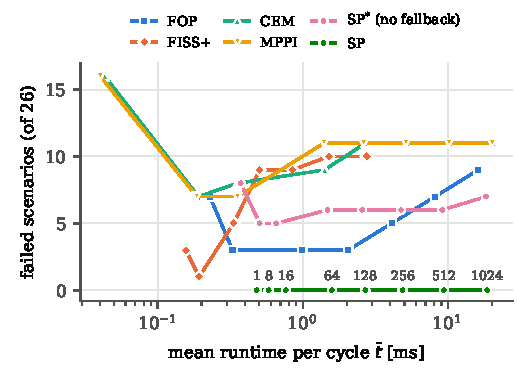
\includegraphics[width=\linewidth]{images/fail_vs_runtime.pdf}
    \caption{Failed scenarios over the average runtime per planning cycle, based on \autoref{tab:planner_comparison}. Each marker is one sample number $N$, increasing from left to right; the labels give $N$ for SP.}
    \label{fig:fail_vs_runtime}
\end{figure}

\subsection{Performance Analysis}
\label{subsec:performance}
\textbf{Reliability.}
As \autoref{tab:planner_comparison} shows, SP completes all 26 scenarios at every sampling number, including $N=1$, and invokes the fallback in only 2.4\% to 3.2\% of the planning cycles.
None of the baselines completes all scenarios at any $N$.
Their failure counts do not decrease monotonically with $N$ but reach a minimum at a moderate sampling number and grow again: FOP fails in 3 scenarios for $N$ between 18 and 125 but in 9 scenarios at $N=990$, FISS+ in 1 scenario at $N=18$ but in 10 scenarios at $N\geq512$, and CEM and MPPI in 11 scenarios for $N\geq128$.
A larger candidate set lets the planner select a lower-cost trajectory in each cycle.
Since each cycle optimizes only its own planning horizon, such choices can lead to states from which no feasible trajectory exists in a later cycle, i.e., inevitable collision states~\cite{Fraichard2004ICS}; in AUT\_Haag-15\_1\_T-9, for example, FOP brakes too late, so that no feasible braking trajectory remains.
These failures are not a matter of sampling resolution: three scenarios that FOP fails at $N=125$ remain unsolved with $22^3=10648$ and $35{\times}20{\times}20=14000$ grid candidates.
SP completes these scenarios, while relying on the FOP grid in only a small fraction of the cycles.

SP$^{*}$ isolates the learned sampler.
Without fallback, it completes 18 scenarios at $N=1$ and 19 to 21 scenarios for $N\geq8$, i.e., more than CEM and MPPI at every $N$ and more than FOP for $N\geq512$; all its failures are cycles in which none of the $N$ samples is feasible.
SP and SP$^{*}$ thus play complementary roles: the learned samples drive the vehicle in about 97\% of the cycles and avoid the dead ends of the greedy baselines, and the fallback covers the remaining cycles in which the learned distribution offers no feasible candidate.

\textbf{Trajectory cost.}
On the scenarios completed by all methods, the cost of SP is comparable with that of the baselines.
For $N\leq8$, SP achieves the lowest or second-lowest cost: 43.8 at $N=1$ compared with 44.1 for CEM and MPPI, and 48.8 at $N=8$ compared with 48.5 for FISS+, 51.2 for CEM and MPPI, and 54.4 for FOP.
For $N\geq64$, the baselines converge to costs between 40.8 and 42.3, whereas SP remains 1.1 to 2.7 higher (3\% to 7\%) at 43.0 to 43.5.
The dense baselines thus find slightly cheaper trajectories in the scenarios they complete, while SP trades this small cost difference for completing all scenarios.

\textbf{Runtime.}
\autoref{fig:fail_vs_runtime} relates reliability to runtime.
With $N=8$, SP completes all scenarios in 0.58\,ms per cycle on average, whereas FOP requires 0.33\,ms for its best result of 3 failed scenarios and 16.2\,ms for 9 failed scenarios at $N=990$.
The runtime of SP comprises a nearly constant CVAE inference of about 0.2\,ms and the evaluation of the $N$ samples, which grows linearly with $N$ as for FOP.
A cycle that triggers the fallback additionally evaluates the 125 grid candidates and takes about 3 to 4\,ms for $N\leq64$; since this occurs in about 3\% of the cycles, it increases the average runtime by only about 0.1\,ms compared with SP$^{*}$ for $N\leq128$.

\subsection{Effect of the Learned Sampling Distribution}
\label{subsec:ablation}
To determine what the CVAE contributes beyond an arbitrary proposal combined with the fallback, its samples are replaced by three non-learned samplers that use the same trajectory evaluation and the same fallback:
\emph{Uniform} draws $(d,\dot{s},T)$ uniformly from the sampling ranges of FOP, i.e., random shooting;
\emph{Marginal} draws parameters from the CVAE training targets, i.e., the unconditioned distribution of the optimal parameters;
and \emph{Mean} uses the mean of these targets for all $N$ samples.
\autoref{tab:ablation} reports the completed scenarios and the fallback rate.

\begin{table}[t]
\caption{Learned versus non-learned samplers, each with the FOP fallback.}
\label{tab:ablation}
\centering
\scriptsize
\setlength{\tabcolsep}{2.6pt}
\renewcommand{\arraystretch}{1.1}
\begin{tabular}{llcccccccc}
\toprule
& & \multicolumn{8}{c}{$N$} \\
\cmidrule(lr){3-10}
Metric & Sampler & 1 & 8 & 16 & 64 & 128 & 256 & 512 & 1024 \\
\midrule
\multirow{4}{*}{\shortstack[l]{Completed\\(of 26)}}
& CVAE (SP) & \textbf{26} & \textbf{26} & \textbf{26} & \textbf{26} & \textbf{26} & \textbf{26} & \textbf{26} & \textbf{26} \\
& Uniform   & 26 & 26 & 26 & 26 & 25 & 23 & 19 & 17 \\
& Marginal  & 24 & 26 & 26 & 25 & 25 & 25 & 23 & 24 \\
& Mean      & 26 & 26 & 26 & 26 & 26 & 26 & 26 & 26 \\
\midrule
\multirow{4}{*}{$P_{fb}$ (\%)}
& CVAE (SP) & \textbf{3.2} & \textbf{2.7} & \textbf{2.5} & 2.4 & 2.4 & 2.7 & 3.0 & 3.0 \\
& Uniform   & 27.9 & 9.3 & 5.4 & 4.5 & 3.3 & 3.1 & 2.3 & 1.6 \\
& Marginal  & 24.9 & 6.4 & 3.0 & 0.7 & 1.1 & 0.3 & 0.1 & 0.05 \\
& Mean      & 34.0 & 34.0 & 34.0 & 34.0 & 34.0 & 34.0 & 34.0 & 34.0 \\
\bottomrule
\end{tabular}
\end{table}

At small $N$, the CVAE requires far fewer fallbacks: at $N=1$, its single sample is feasible in 96.8\% of the cycles, compared with 72.1\% for Uniform, 75.1\% for Marginal, and 66.0\% for Mean.
% TODO(author): the same-state feasibility measured along the closed loop of SP (shadow evaluation, N=1) gives 96.6 / 77.8 /
% 73.8 / 71.6 %; the numbers above are 100 - P_fb of the closed-loop runs. Use one of the two consistently.
The advantage is not explained by the distribution of good parameters alone, since Marginal and Mean draw on the same training targets without the scene context; it therefore stems from conditioning on the BEV input.

At large $N$, the non-learned samplers reach lower fallback rates than the CVAE, but lose scenarios even though the fallback is available: Uniform fails in 9 scenarios at $N=1024$, eight of which are also failed by FOP at $N=990$.
With many samples spread over the full parameter range, selecting the lowest-cost candidate reproduces the greedy behavior of the dense baselines, and the vehicle enters states in which neither the samples nor the fallback grid contain a feasible trajectory.
The CVAE samples remain concentrated in the learned region of the parameter space, so that a larger $N$ refines the choice within this region rather than toward the aggressive extremes.
This explains the trend of $P_{fb}$ in \autoref{tab:planner_comparison}: from $N=1$ to $N=64$, the fallback rate decreases because more samples make a feasible candidate more likely; beyond $N=64$, it increases slightly from 2.4\% to 3.0\% as the lower-cost selection drives the vehicle into tighter situations more often, which the fallback resolves without losing any scenario.
% TODO(author): the last explanation is supported by the closed-loop outcomes but not yet by a direct measurement (e.g., the
% minimum time gap before the fallback cycles at N=128 versus N=1024). Soften to "is consistent with" if not added.

\textbf{Generalization to unseen maps.}
On the 11 scenarios whose road maps do not occur in the training data, SP completes all scenarios for $N=1$, 8, and 64 with fallback rates of 1.7\%, 0.9\%, and 0.9\%, compared with 37.0\%, 15.7\%, and 7.4\% for Uniform and 30.6\%, 8.7\%, and 1.6\% for Marginal, which additionally fails in one scenario at $N=64$.
Without fallback, SP$^{*}$ completes 8, 10, and 10 of these scenarios, compared with 2, 3, and 5 for Uniform, 1, 3, and 6 for Marginal, and 6 to 10 for FOP across all its grids.
The learned scene-conditioned prior thus transfers to road layouts not seen during training.

\subsection{Qualitative Case Study}
\label{subsec:case_study}
% TODO(author): Fig. 3 and this subsection come from the earlier Python runs on scenarios outside the 26 evaluation scenarios
% (USA_NewYork-54_1_T-1, CHN_Qingdao-5_37_T-1). Regenerate the figure with the current C++ planners (SP N=64, FOP/FISS+ N=125)
% or replace it by a scenario of the evaluation set, e.g. AUT_Haag-15_1_T-9, which FOP, FISS+, CEM and MPPI fail at every N
% while SP completes it. The text below keeps only statements that the figure can show.
To illustrate the behavioral differences under challenging traffic conditions, \autoref{fig:scenario_brake} shows two representative scenarios.

The scenario in \autoref{fig:newyork} is a lane-following scenario with a dynamic obstacle ahead of the ego vehicle.
At time steps 50 and 80, SP keeps a larger longitudinal clearance from the leading vehicle than FOP and FISS+.
The CVAE is trained on the trajectory parameters selected by FOP with a dense grid of 19040 candidates (\autoref{subsec:dataset}), which cannot be evaluated in real time; SP reproduces part of this behavior with 64 samples.

The scenario in \autoref{fig:qingdao} is a drive-brake-drive maneuver, which violates the assumption of the FISS+ heuristic that the solution of the next cycle is close to that of the previous one.
At time step 63, FISS+ fails to find a feasible trajectory: it selects low-cost trajectories near its previous solution with insufficient deceleration, so that the ego vehicle approaches the stopping leading vehicle too closely and no braking trajectory remains feasible.
FOP and SP complete the scenario, and SP keeps a larger distance from the leading vehicle, particularly at time step 100.
